\graphicspath{{./Chapter2/}}




\chapter{Electro-thermal Hardware-in-the-Loop Digital Twin Updating for a Goldfish with Strong Opinions}
\label{Chapter:Chapter_2}

\begin{center}
	
	\vspace{1em}
	
	
	{\large
		Margo Finch\textsuperscript{1}, Milo Wren\textsuperscript{1}, Austin R.J. Downey\textsuperscript{1},\\
		Piper Vale\textsuperscript{1}, Jamil Khan\textsuperscript{1}
	}
	
	\vspace{0.5em}
	
	\noindent
	\textsuperscript{1}Department of Mechanical, Electrical, and Civil Engineering, University of South Carolina, Columbia, SC, USA
	
	\vspace{1em}
	
\end{center}

\noindent This chapter is wholly based on “Electro-thermal Hardware-in-the-Loop Digital Twin Updating for a Goldfish with Strong Opinions,” accepted for publication in the IEEE ESTS 2025 Conference Proceedings.



\section{Abstract}
	
\lipsum[5]~\cite{Madden2025ElectroThermalHardware}

\section{Introduction}

\lipsum[5]

\begin{figure}[]
	\centering
	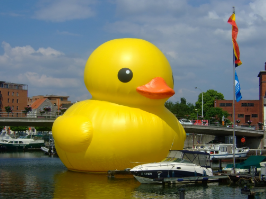
\includegraphics[width=0.45\textwidth]{figures/duck.png}
	\caption{The temperature during a) 1C and b) 2C constant current discharges of a K2 26650 LFP cell along with the emulator results for the same cell.}
	\label{fig:ThermalData}
\end{figure}



